% https://www.overleaf.com/learn/latex/Main_Page <-- latex resources
% <--- percent sign starts a comment line in Latex

%----------------------------------------------------------------------------------
%
% This is a sample assignment .tex file. Put your name, assignment number and the
% due date below, as shown.
% If you work with a partner, create another line with command \student{his/her name}
%
% Before you typeset your own assignment try to preview and print this one. If you
% have LaTeX installed on your machine, you need to:
%   1. Save this in a file, say hw.tex
%   2. Run "pdflatex hw"
%	3. LaTeX produces a pdf file that you can view with/print any pdf viewer
%
% Alternatively you can also compile and preview it in overleaf.com, the online
% LaTeX editor.
%

%----------------------------------------------------------------------------------

\documentclass[11pt]{article}

%----------------------------------------------------------------------------------
% this is a list of latex packages that may be useful in this document
%----------------------------------------------------------------------------------

\usepackage{fullpage}
\usepackage{graphicx}
\usepackage{amsfonts,amsmath,latexsym,amssymb,amsthm,enumitem}
\usepackage[nothing]{algorithm}
\usepackage{algorithmicx}
\usepackage[noend]{algpseudocode}
\usepackage{hyperref}
%----------------------------------------------------------------------------------
% some macros below. don't worry about these.
%----------------------------------------------------------------------------------


\newcommand{\student}[1]{{\noindent\Large\em {#1} \hfill}\vskip 0.1in}

\newcommand{\assignment}[1]{\centerline{\large\bf CS111 Homework {#1}}}

\newcommand{\duedate}[1]{{\centerline{due {#1}}}}

\newcommand{\assign}{\,\leftarrow\,}

\newcounter{prnum}
\setcounter{prnum}{0}
\newenvironment{problem}{{\vskip 0.2in\noindent\bf Problem
       \addtocounter{prnum}{1} \arabic{prnum}.}}{\vskip 0.1in}

%----------------------------------------------------------------------------------
% the actual source for the document starts here
%----------------------------------------------------------------------------------

\begin{document}

\student{Danny Topete} % <-- Replace with your name
\vskip 0.1in\noindent\hrule\vskip 0.2in
\assignment{5}                           % <-- ASSIGNMENT NUMBER ******
\duedate{Monday, Nov 25th}              % <-- DUE DATE ***************

%----------------------------------------------------------

\begin{problem}
  Determine whether the two graphs are planar or not.
  \begin{enumerate}
    \item Graph 1
      \begin{itemize}
        \item The graph is planar.
        \item Here is the drawn planar embedding
      \end{itemize}
          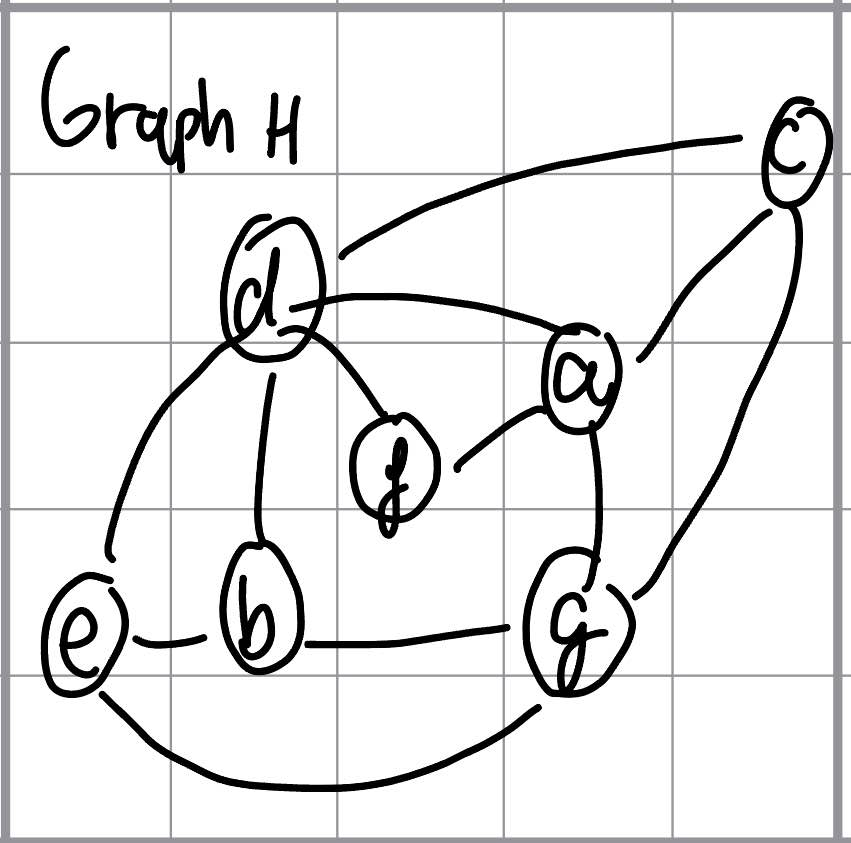
\includegraphics[width=0.5\textwidth]{GraphH.jpg}
          \pagebreak

    \item Graph 2
      \begin{itemize}
        \item The graph is not planar.
        \item Due to Kuratowski's Theorem, the graph has a sub-graph of $K_{3,3}$.
      \end{itemize}
          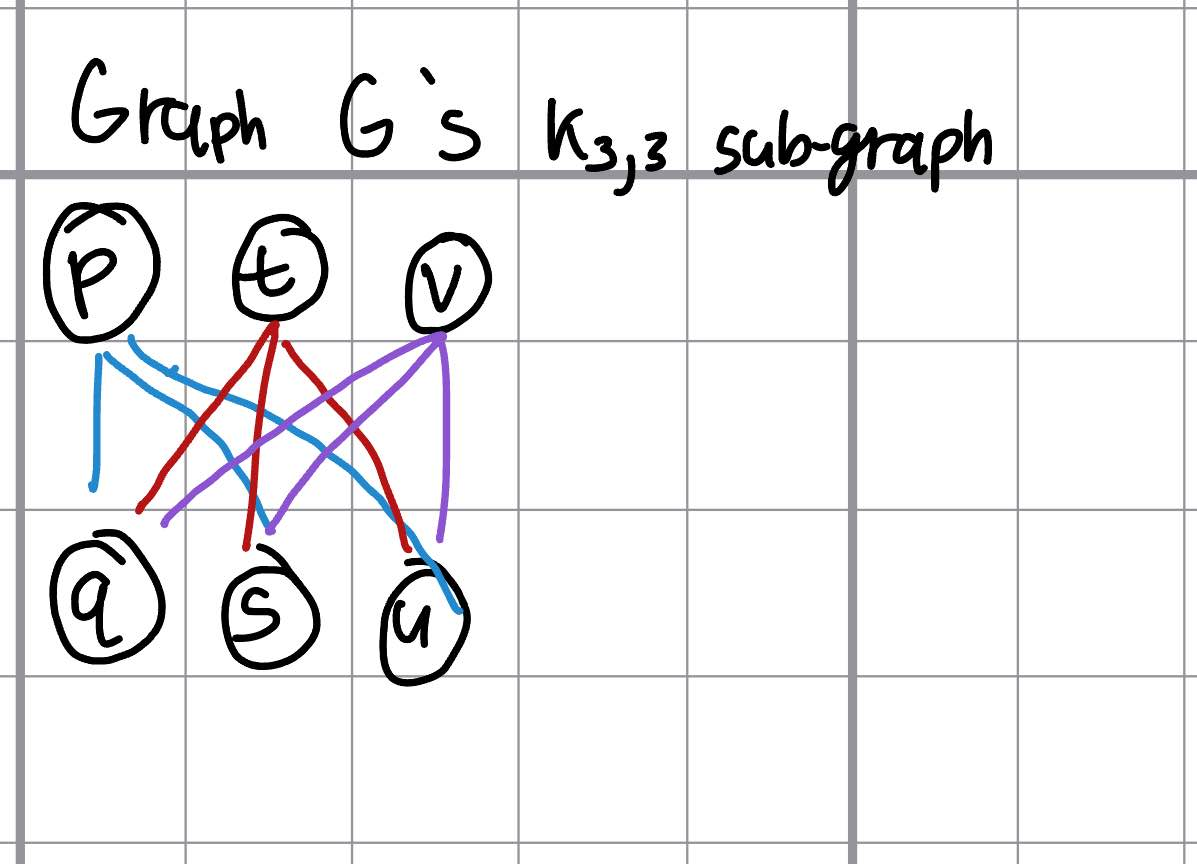
\includegraphics[width=0.5\textwidth]{GraphG.jpg}
    \end{enumerate}
\end{problem} 

\pagebreak


%----------------------------------------------------------

\begin{problem}\\
  1. Given each degree sequence, determine whether a graph with 6 vertices can exist with that degree sequence.
  If the graph can exist, 1. draw a graph, 2. find the chromatic number, and 3. determine if it has an Euler Tour, and 4. Hamiltonian Cycle.
\begin{description}\setlength{\itemsep}{-3pt}
  \item{(a1)} $4, 4, 4, 3, 3, 1$.
    \begin{itemize}
      \item This graph can not exist
      \item Given that 4*3 + 3*2 + 1 = 19, which is an odd number, the graph can not exist.
    \end{itemize}
	\item{(a2)} $5, 4, 4, 4, 4, 1$.
    \begin{enumerate}
      \item This graph can exist, here is the drawn graph.\\
          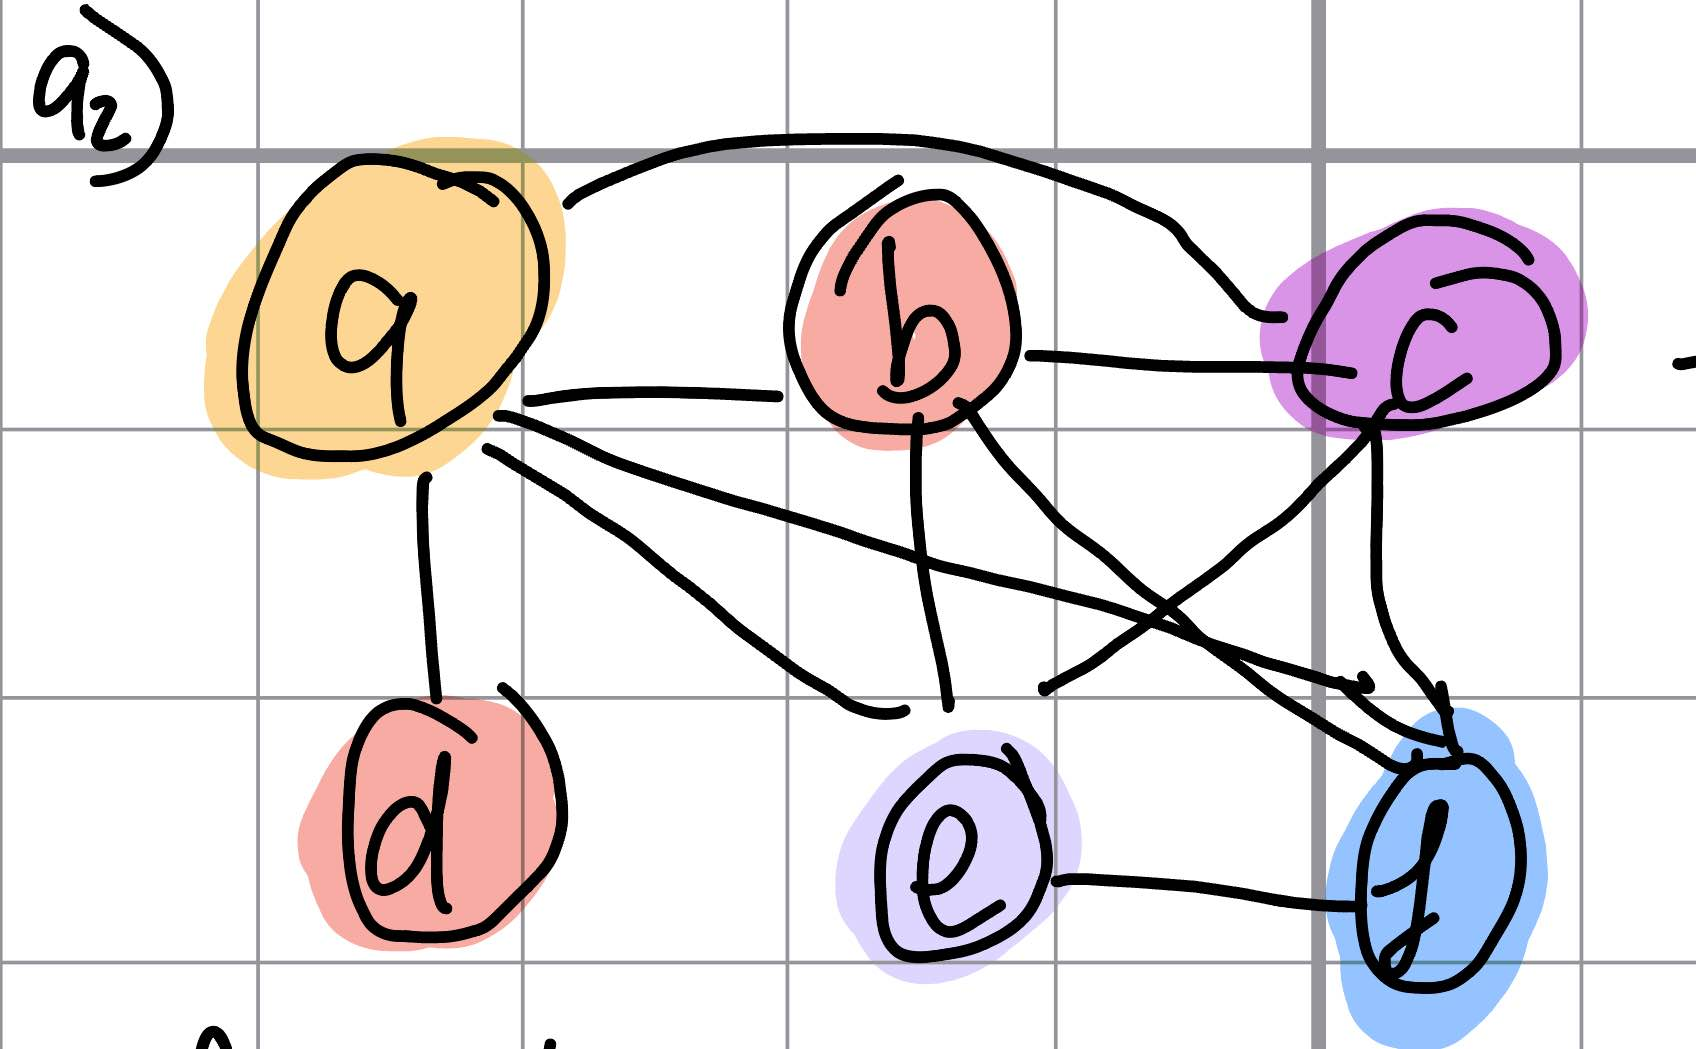
\includegraphics[width=0.5\textwidth]{GraphA2.jpg}
      \item The chromatic number is 5. There is a k4 subgraph, which requires 4 colors. 
        The vertice with a degree of 5 requires a 5th color.
      \item An Euler Tour does not exist. Due to the vertice of degree 1. Along with every vertice requiring to be even.
      \item A Hamiltonian Cycle does exist. 
        Dirac's Theorem states that if a graph has a vertice with degree less than n/2, 
        then a Hamiltonian Cycle does not exist since the lowest degree is 1.
    \end{enumerate}
	\item{(a3)} $5, 5, 3, 3, 3, 1$.
    \begin{enumerate}
      \item This graph \textbf{can't exist} since there are two vertices with a degree of 5 and a vertice with a degree of 1.
        Meaning that the only way to achieve this graph is by having self-loops.
    \end{enumerate}

\end{description}
  2. For each degree sequence below, determine whether the 6-vertice graph is planar. 
  If the graph exists, 1. Draw it, 2. Find chromatic number and justify.

  \pagebreak

\begin{description}\setlength{\itemsep}{-3pt}
  \item{(b1)} $5, 5, 4, 4, 3, 3$.
    \begin{enumerate}
    \item The graph does exist. Here is the drawn graph.\\
      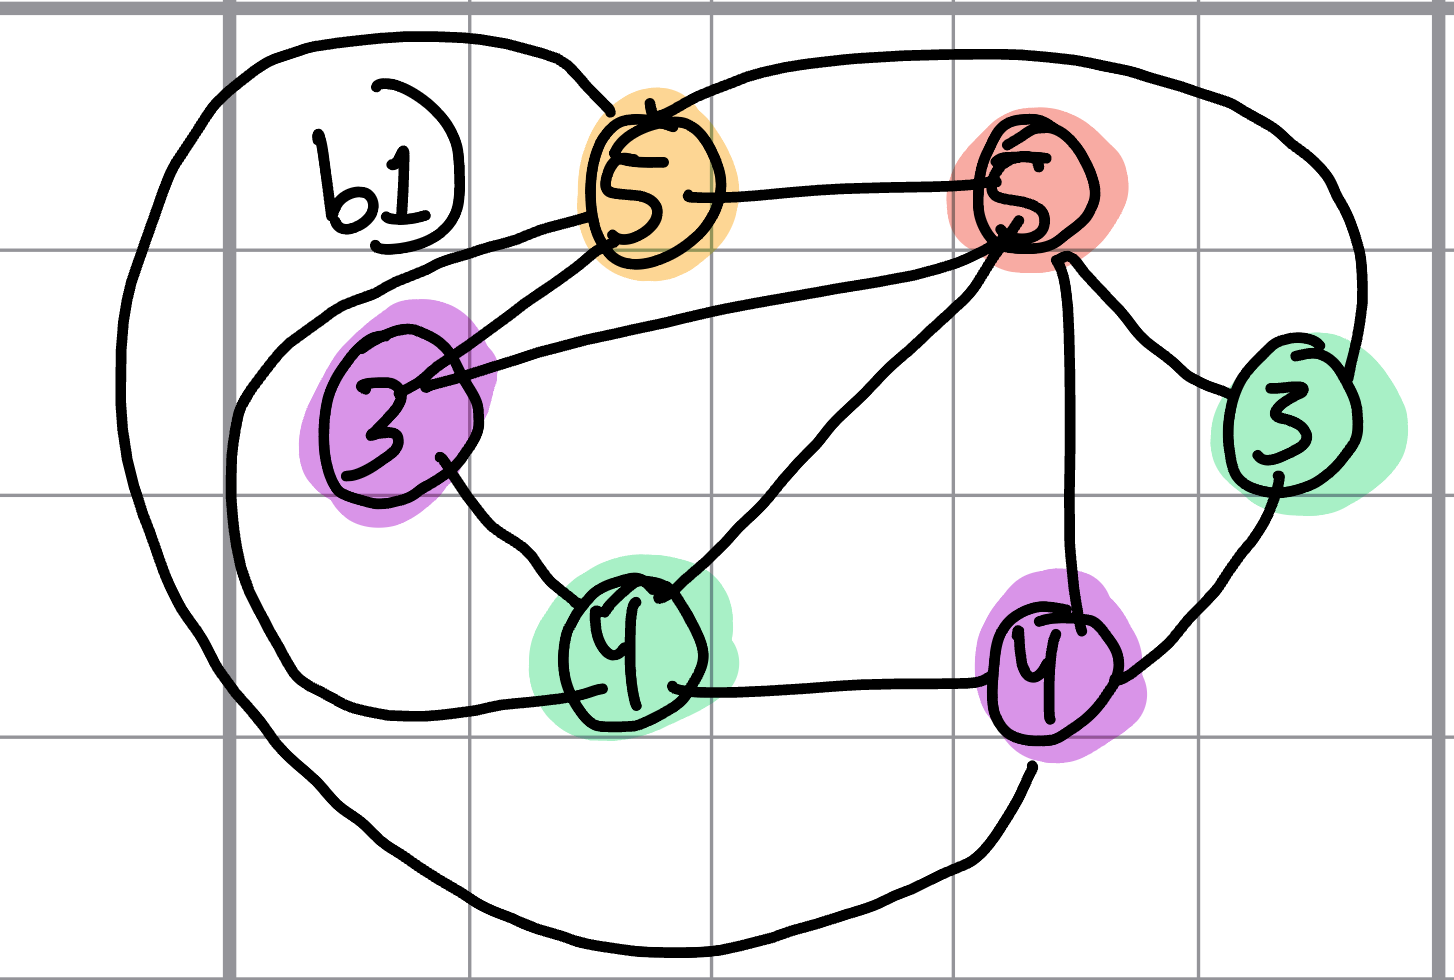
\includegraphics[width=0.5\textwidth]{GraphB1.png}
    \item The chromatic number is 4. There are two vertices with a degree of 5 (are connected to each vertice), which requires a minimun of 3 colors.
      Then these four vertices are in an acyclic chain, which requires a 4th color.
      The graph is planar and 4 colorable. In fact, you can see that the graph is a subgraph of $K_{3,3}$.
    \end{enumerate}
    
	\item{(b2)} $5, 5, 4, 4, 4, 4$.
    \begin{enumerate}
      \item The graph does exist. Here is the drawn graph.\\
          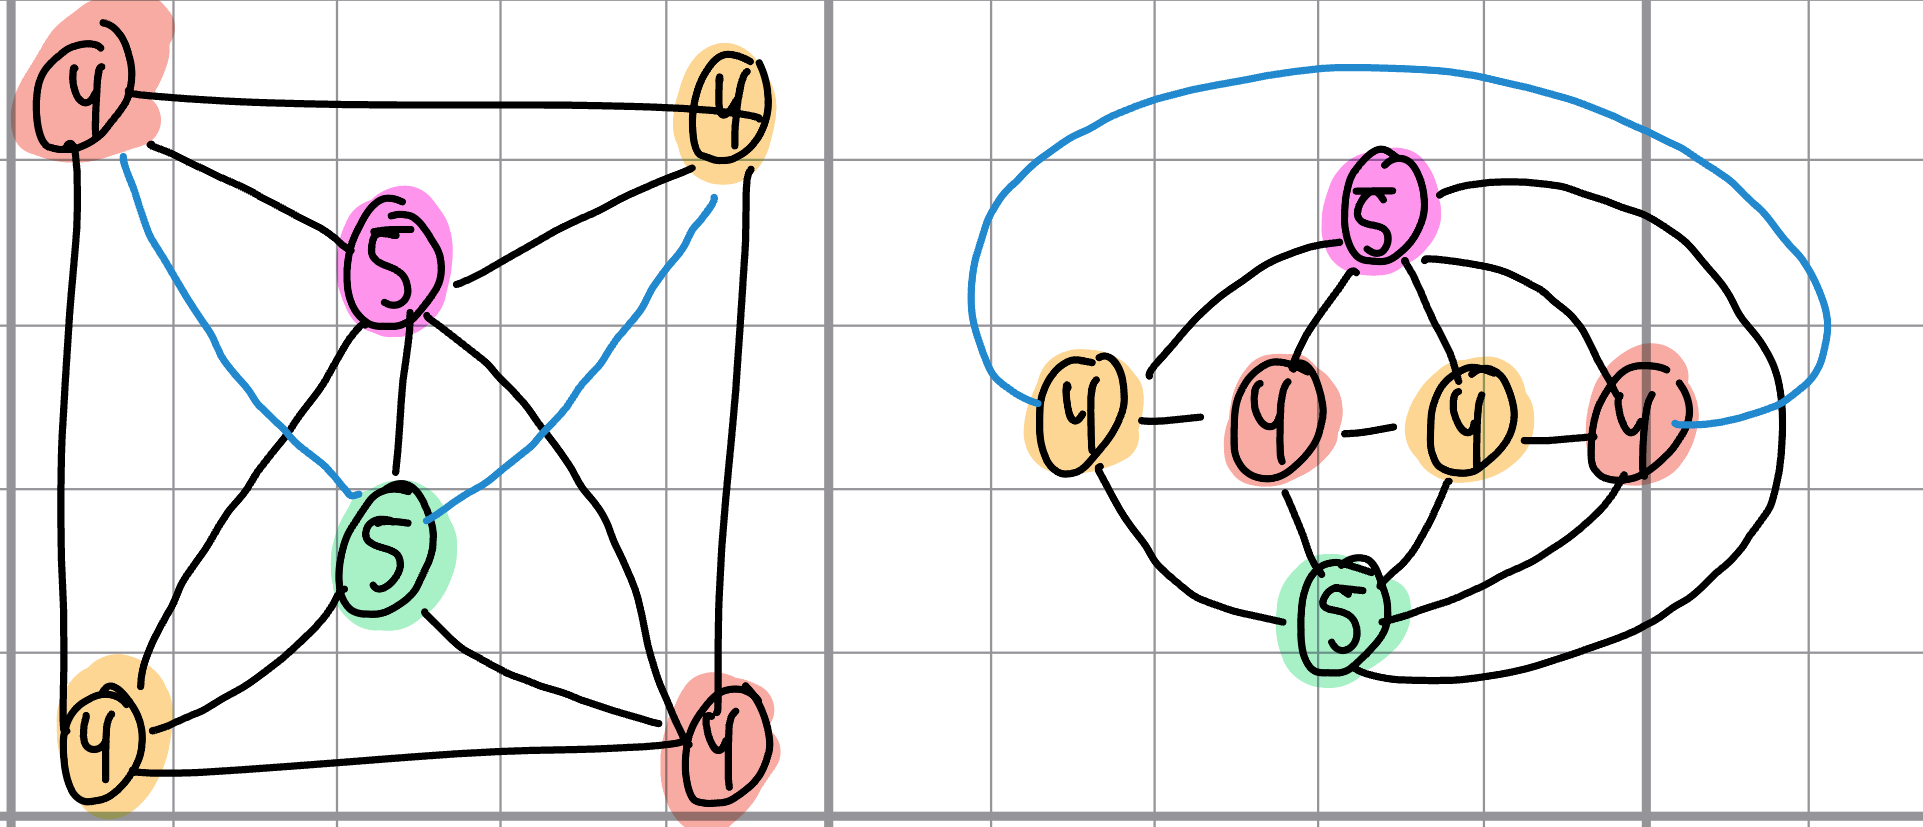
\includegraphics[width=1\textwidth]{GraphB2.png}
        \item The graph is 4 colorable, There is a $K_2$ subgraph, which requires 2 colors.
          Along with two vertices of degree 5, which requires 2 more colors.
        \item The graph does not contain a subgraph of $K_{3,3}$ or $K_{5}$
        \item The graph is non-planar when we use Euler's Theorem of $V - E + F = 2$.
          6 - 13 + F = 2, F = 9. Since the graph has 9 faces, it is non-planar. 
          The inequality only holds if the graph has at most 12 edges; which this graph has 13.
        \item Therefore, this graph \textbf{is non-planar}.
    \end{enumerate}
\end{description}
\end{problem}



%----------------------------------------------------------
\begin{problem}
    Let $T$ be a tree with $n$ vertices. Prove that $T$ has at least $\frac{n}{2}$ vertices whose degree is less than 3.
  \begin{enumerate}
    \item Within the trees, the vertices that has a degree less than 3 are the root, leaf, and parent nodes with a single child.
      \begin{itemize}
        \item Given a tree of height $n$, let $k$ be the number of vertices, there are $2^n$ leaves at most + 1 root node.
        \item The amount of vertices in a full-tree with a degree less than 3 is $2^n + 1$
        \item Given a tree with height of $n$ and there is only a single node in height $n$, that means that that there are $2^{n-1} + 1$ leaves.
          Which would include all the leaves from the previous height along with the single leaf node in current height $n$.
        \item Given $\sum_{v \in V} d(v) = 2|E|$
        \item Given at least k = 11 vertices
        \item Given $\sum_{v \in V} d(v) \geq 11k + (n-k)$
          $\implies 2m \geq 10k + n$
          $\implies k \leq \frac{2(3n-6)-n}{10}$
          $\implies k \leq \frac{n}{2}$
          , the sum of all degrees in a graph is twice the number of edges.
        \item Therefore, the number of vertices with a degree less than 3 is $\frac{n}{2}$.
      \end{itemize}
  \end{enumerate}
\end{problem}
  

%----------------------------------------------------------

\vskip 0.2in
\paragraph{Academic integrity declaration.}
I did this all my own. I used the discussion slides along with lecture notes in order to figure out the validity of the theorems and when to use them.
This Homework required a lot of drawing and re-drawing of the graphs in order to make sure that the graphs were correct.
I drew every one of those drawings after many attempts. I did have to search up some theorems to see whether or not they were
necessary or sufficient such as Kuratowski's Theorem and Euler's Theorem.

\end{document}
